\documentclass[12pt,t]{beamer}
\subtitle{1 -- Introduction}
\usepackage{graphicx}
\setbeameroption{hide notes}
\setbeamertemplate{note page}[plain]

% get rid of junk
\usetheme{default}
\beamertemplatenavigationsymbolsempty
\hypersetup{pdfpagemode=UseNone} % don't show bookmarks on initial view

% font
\usepackage{fontspec}
\setsansfont{TeX Gyre Heros}
\setbeamerfont{note page}{family*=pplx,size=\footnotesize} % Palatino for notes
% "TeX Gyre Heros can be used as a replacement for Helvetica"
% In Unix, unzip the following into ~/.fonts
% In Mac, unzip it, double-click the .otf files, and install using "FontBook"
%   http://www.gust.org.pl/projects/e-foundry/tex-gyre/heros/qhv2.004otf.zip

% named colors
\definecolor{offwhite}{RGB}{249,242,215}
% \definecolor{foreground}{RGB}{255,255,255}
\definecolor{foreground}{RGB}{0,0,0}
% \definecolor{background}{RGB}{24,24,24}
\definecolor{background}{RGB}{255,255,255}
\definecolor{title}{RGB}{107,174,214}
\definecolor{gray}{RGB}{100,100,100}
\definecolor{subtitle}{RGB}{102,155,204}
\definecolor{hilight}{RGB}{20,180,204}
\definecolor{vhilight}{RGB}{255,111,207}
\definecolor{lolight}{RGB}{155,155,155}
%\definecolor{green}{RGB}{125,250,125}

% use those colors
\setbeamercolor{titlelike}{fg=title}
\setbeamercolor{subtitle}{fg=subtitle}
\setbeamercolor{institute}{fg=gray}
\setbeamercolor{normal text}{fg=foreground,bg=background}
\setbeamercolor{item}{fg=foreground} % color of bullets
\setbeamercolor{subitem}{fg=gray}
\setbeamercolor{itemize/enumerate subbody}{fg=gray}
\setbeamertemplate{itemize subitem}{{\textendash}}
\setbeamerfont{itemize/enumerate subbody}{size=\footnotesize}
\setbeamerfont{itemize/enumerate subitem}{size=\footnotesize}

% settings for table of contents
\setbeamercolor{section in toc}{fg=foreground,bg=background}
\setbeamerfont{subsection in toc}{size=\footnotesize}
\setbeamertemplate{section in toc}{{\scriptsize\leavevmode\raise1.35pt\hbox{$\blacktriangleright$}} \inserttocsection}
%\setbeamertemplate{subsection in toc}{\quad{\tiny\leavevmode\raise1.5pt\hbox{$\blacktriangleright$}} \footnotesize\inserttocsubsection\\}
\setbeamertemplate{subsection in toc}{\quad\quad\textendash\enspace\inserttocsubsection\\}

% page number
\setbeamertemplate{footline}{%
    \raisebox{5pt}{\makebox[\paperwidth]{\hfill\makebox[20pt]{\color{gray}
          \scriptsize\insertframenumber}}}\hspace*{5pt}}

% add a bit of space at the top of the notes page
\addtobeamertemplate{note page}{\setlength{\parskip}{12pt}}

% add subsection as frame title when it is empty
\makeatletter
  \CheckCommand*\beamer@checkframetitle{%
    \@ifnextchar\bgroup\beamer@inlineframetitle{}}
  \renewcommand*\beamer@checkframetitle{%
    \global\let\beamer@frametitle\relax\@ifnextchar%
    \bgroup\beamer@inlineframetitle{}}
\makeatother

\addtobeamertemplate{frametitle}{
  \ifx\insertframetitle\empty
      \frametitle{\insertsubsectionhead}
  \else
  \fi
 }{}


\usepackage{pbox}

% a few macros
\newcommand{\bi}{\begin{itemize}}
\newcommand{\ei}{\end{itemize}}
\newcommand{\ig}{\includegraphics}
\newcommand{\subt}[1]{{\footnotesize \color{subtitle} {#1}}}

% title info
\title{Kompetitives Programmieren}
%\author{Gregor Behnke}
\institute{Prof. Dr. Susanne Biundo-Stephan \\ Gregor Behnke \\ Institute of Artificial Intelligence\\ Ulm University}
\date{\tiny based on Bjarki Ágúst Guðmundsson's and Tómas Ken Magnússon's\\Competitive Programming}


\setbeamertemplate{footline}[text line]{%
  \parbox{\linewidth}{\vspace*{-8pt}\shorttitle \hfill \insertframenumber/\inserttotalframenumber}}
\setbeamertemplate{navigation symbols}{}


\newcommand{\specialcell}[2][c]{%
  \begin{tabular}[#1]{@{}c@{}}#2\end{tabular}}

% Tikz
\usepackage{tikz}
\usepackage{tkz-euclide}
\usetikzlibrary{arrows,shapes}
% \usepackage{intersections}
\usetkzobj{all}
\usetikzlibrary{arrows,shapes,angles,quotes,shapes, calc, decorations,matrix}
\usepackage{forest}
\pgfdeclarelayer{bg}    % declare background layer
\pgfsetlayers{bg,main}


% Minted
\usepackage{minted}
\usemintedstyle{tango}
\newminted{cpp}{fontsize=\footnotesize}

% Graph styles
\tikzstyle{vertex}=[circle,fill=black!50,minimum size=15pt,inner sep=0pt, font=\small]
\tikzstyle{selected vertex} = [vertex, fill=red!24]
\tikzstyle{selected2 vertex} = [vertex, fill=hilight!50, text=black]
\tikzstyle{vertex1} = [vertex, fill=red]
\tikzstyle{vertex2} = [vertex, fill=blue]
\tikzstyle{vertex3} = [vertex, fill=green, text=black]
\tikzstyle{vertex4} = [vertex, fill=yellow, text=black]
\tikzstyle{vertex5} = [vertex, fill=pink, text=black]
\tikzstyle{vertex6} = [vertex, fill=purple]
\tikzstyle{edge} = [draw,thick,-]
\tikzstyle{dedge} = [draw,thick,->]
\tikzstyle{weight} = [font=\scriptsize,pos=0.5]
\tikzstyle{selected edge} = [draw,line width=2pt,-,red!50]
\tikzstyle{ignored edge} = [draw,line width=5pt,-,black!20]


\begin{document}

% title slide
{
    \setbeamertemplate{footline}{} % no page number here
    \frame{
        \titlepage
    }
}




% TODO: Welcome
\begin{frame}{What is Competitive Programming?}
    \vspace{40pt}
    \bi
		\item .. the art of solving complex, well-defined algorithmical or mathematical problems quickly within a given time-bound (both for coding and program runtime) 

		\vspace{20pt}
		\pause
		\item There are a \emph{lot} of Programming Competitions
		\bi
			\item Google Code Jam
			\item Facebook Hacker Cup
			\item IOI
			\item HackerRank
			\item TopCoder
			\item ACM ICPC

		\ei
    \ei
\end{frame}

\begin{frame}{What is the ACM ICPC?}
\vspace{20pt}
\bi
\item Annual, multi-level programming contest for students
\item Students participate in teams of 3 and share a single computer
\item 5 hours and 10-12 programming problems
\pause
\vspace{20pt}
\item The team with the most solved problems wins!
\pause
\vspace{20pt}
\item Multi-level competition
		\bi
			\item GCPC (German Collegiate Programming contest) - June/July
			\item NWERC (North-Western European Regional Contest) - End of November
			\item World Finals - March - June
		\ei
\ei
\end{frame}

%\begin{frame}{What is the ACM ICPC?}
%		\begin{center}
%			\only<1>{\includegraphics[width = 0.95\textwidth]{images/hall.jpg}}
%			\only<2>{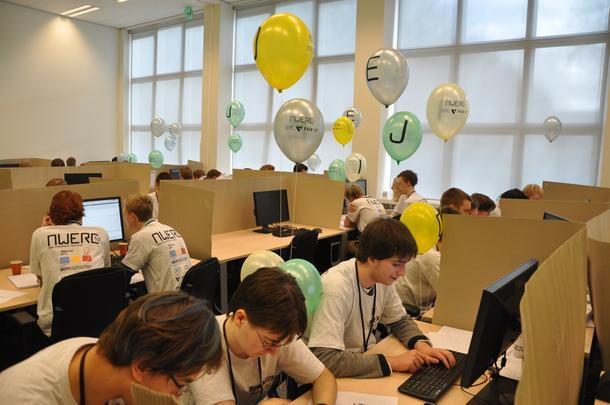
\includegraphics[width = \textwidth]{images/team.jpg}}
%			\only<3>{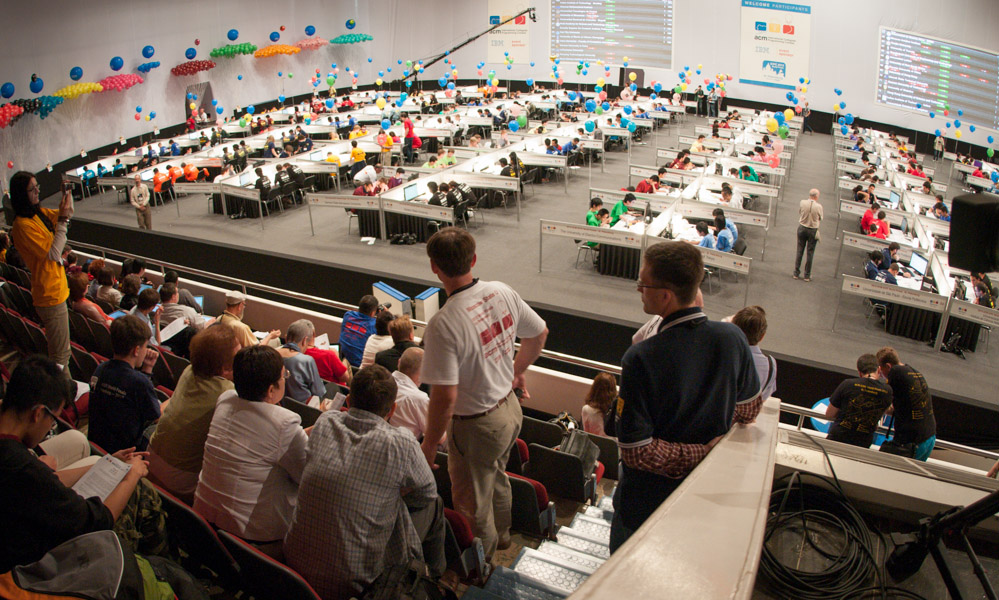
\includegraphics[width = \textwidth]{images/wf.jpg}}
%			\only<4>{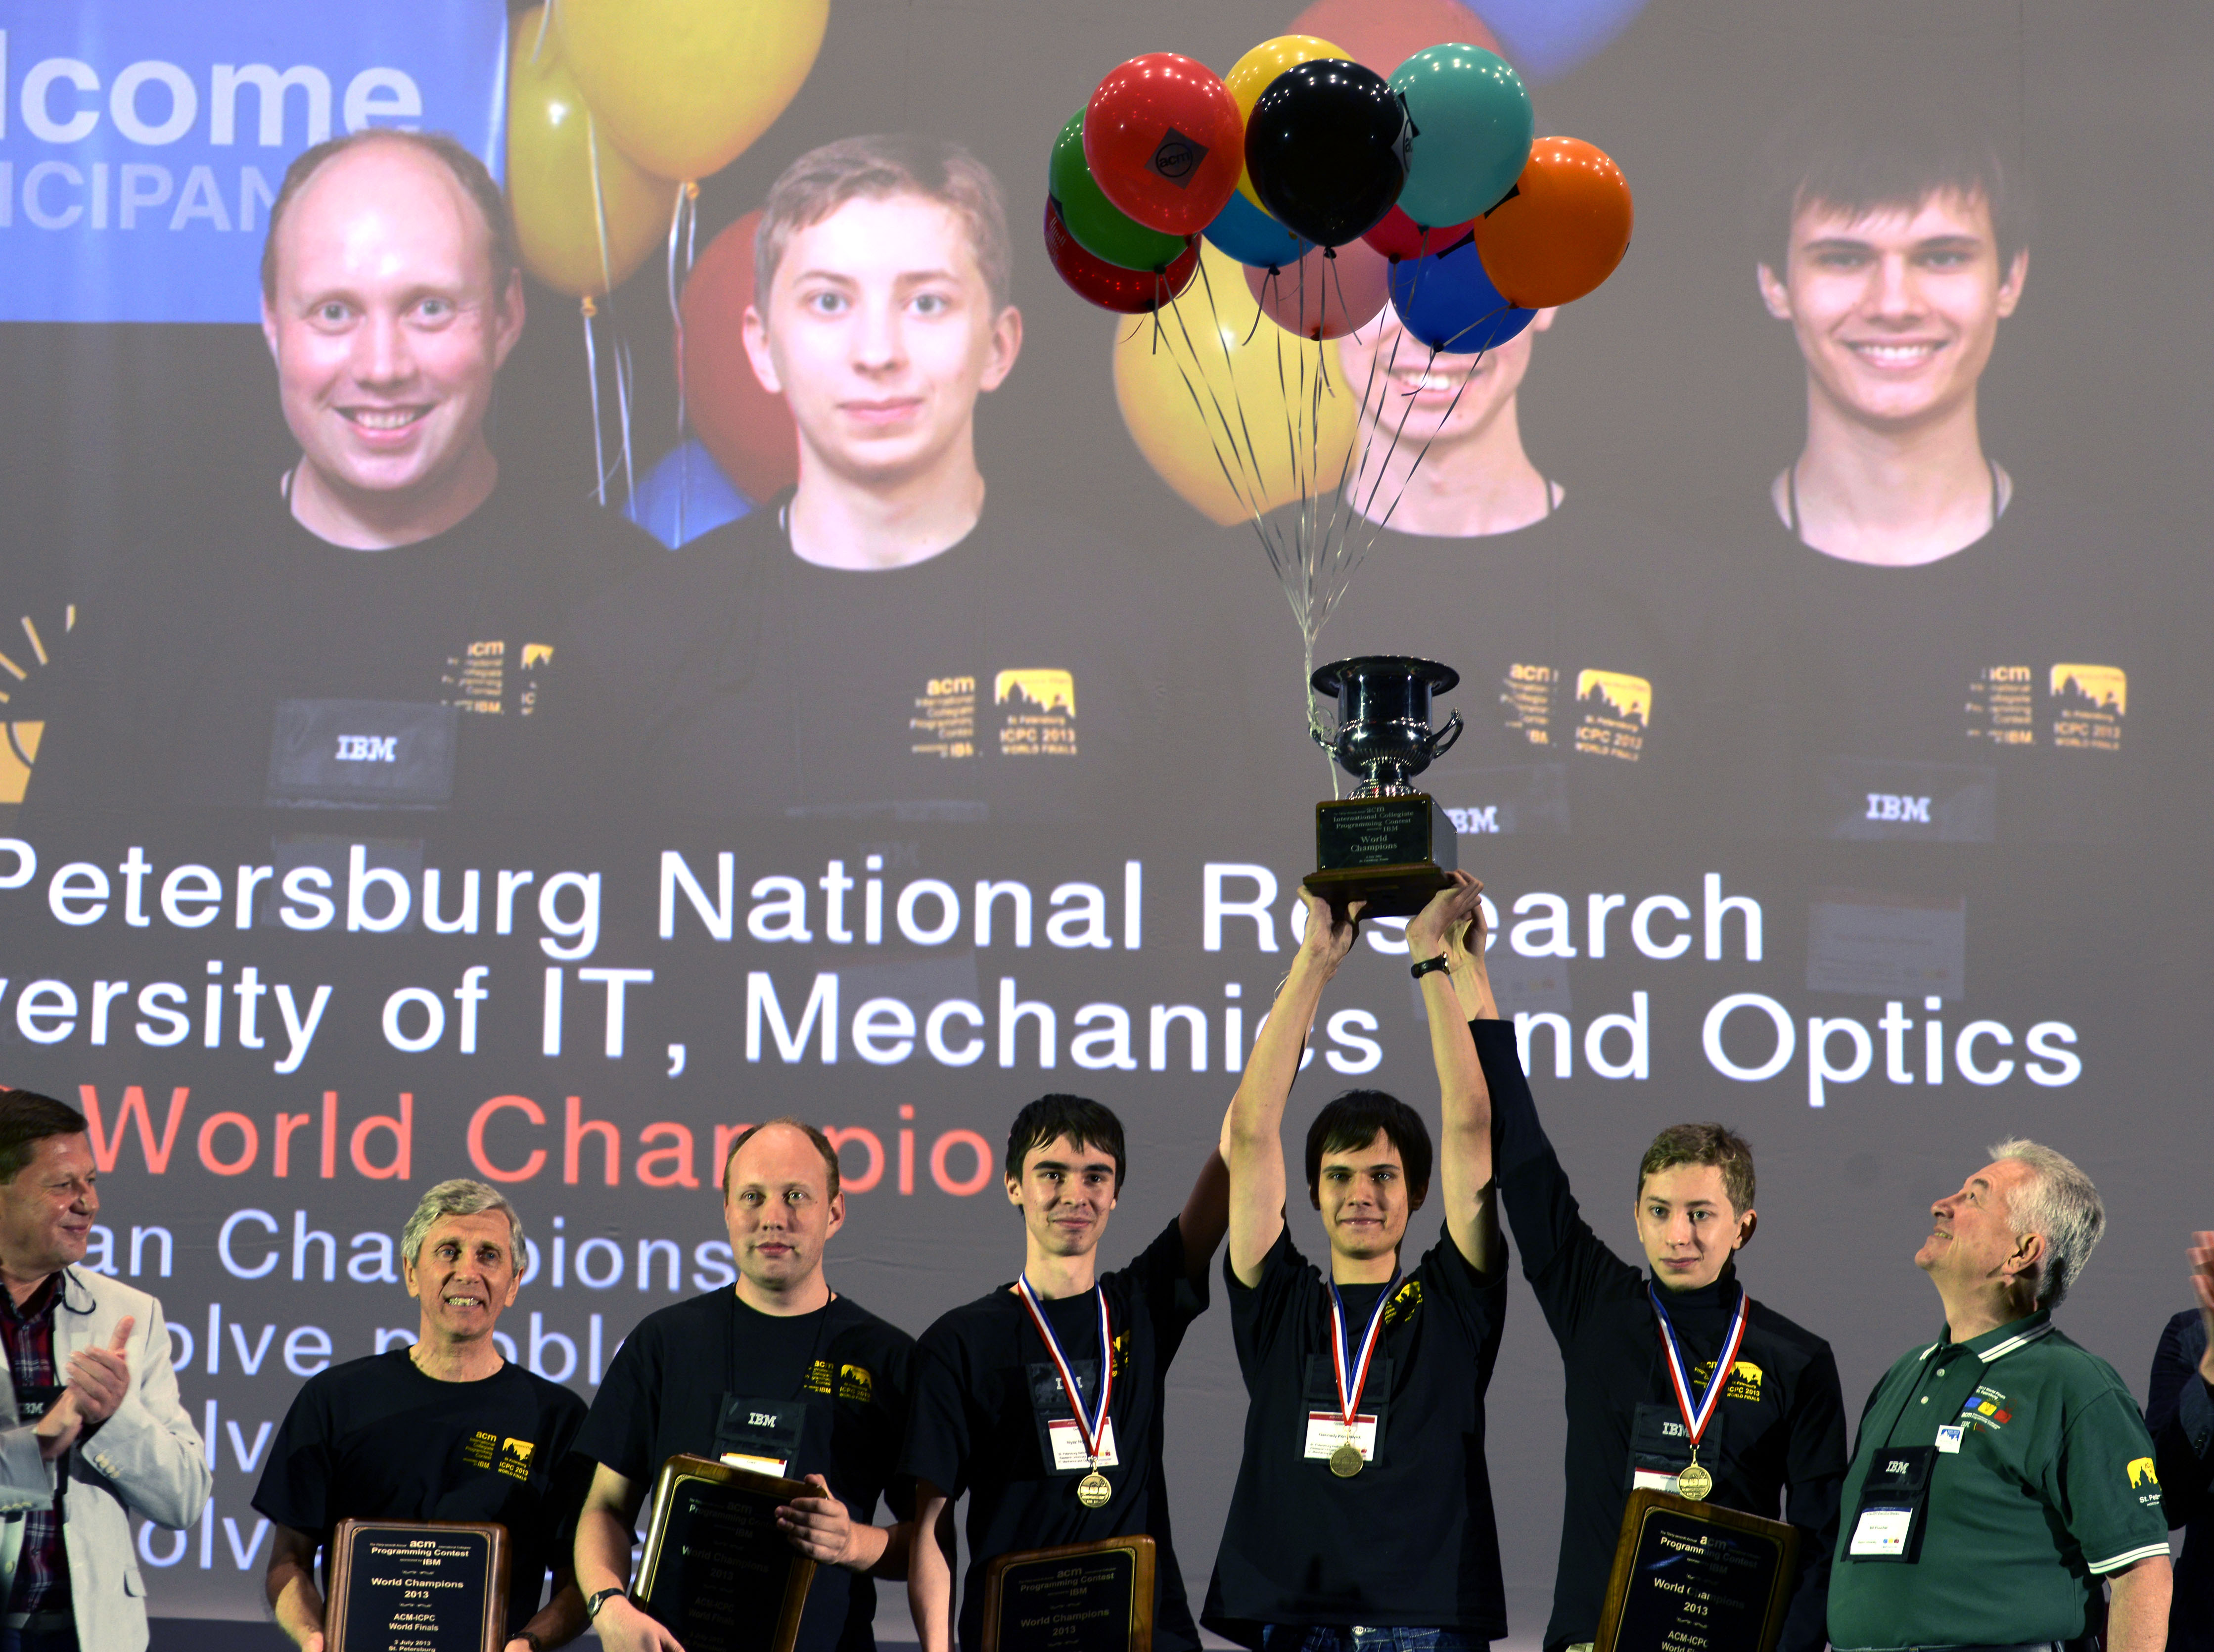
\includegraphics[width = 0.95\textwidth]{images/wc.jpg}}
%			\only<5>{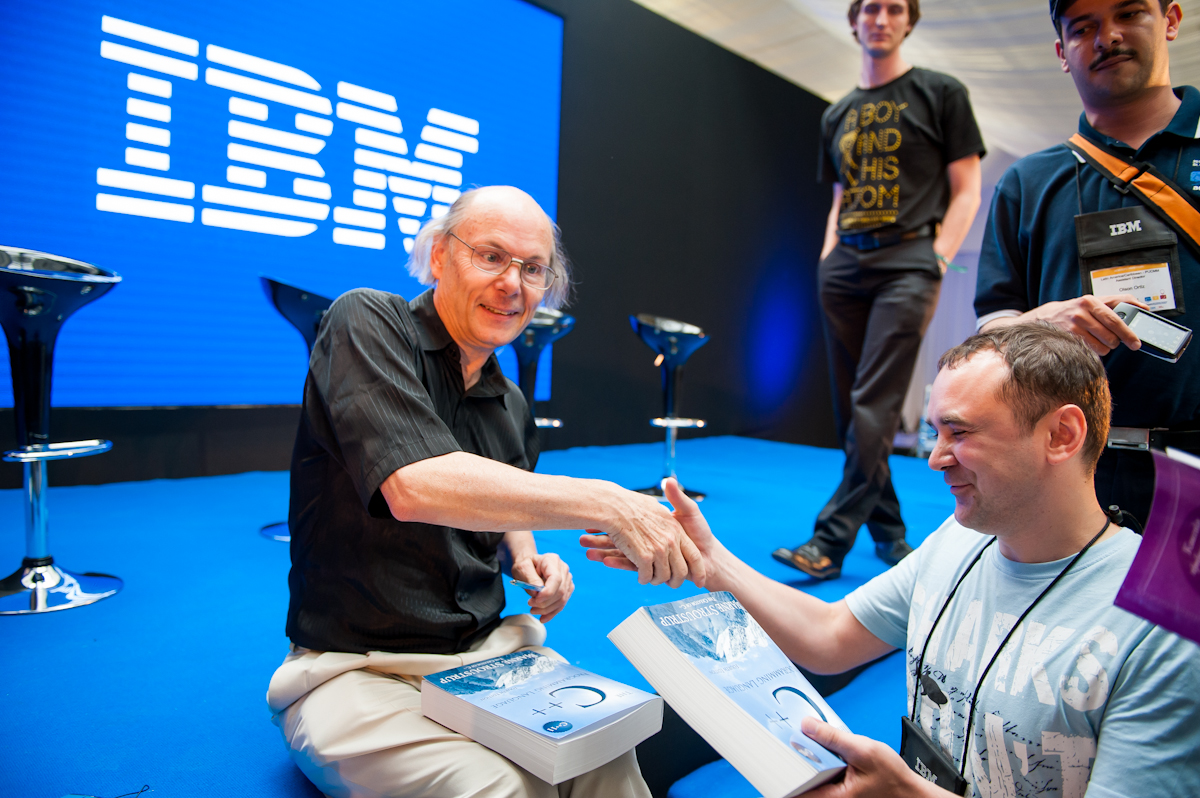
\includegraphics[width = \textwidth]{images/bjarne.jpg}}
%		\end{center}
%\end{frame}

\begin{frame}{Why train Competitive Programming?}
    \bi
		\item Learn about new algorithms.
		\item Learn to tackle complex problems in a systematic way.
		\item Learn to see patterns in problems.
		\item Learn perseverance when facing (seemingly) impossible problem.
		\item Learn to de-bug problems.
		\item Learn to design algorithms that always work.

		\pause \vspace{10pt}
		\item To be a better (and faster) programmer!
		\pause \vspace{10pt}
		\item To succed at job interviews!
		\pause \vspace{10pt}
		\item To win programming competitions!
	\ei
\end{frame}
        
% TODO: Goals
\begin{frame}{Goal}

    \vspace{30pt}

    \bi
        \item Given a problem, we want to
            \bi
                \item solve it efficiently
                \item by using algorithms and data structures,
                \item convert our solution into a program,
                \item do it as quickly as possible (under pressure)
                \item and do it correctly (without bugs)
            \ei

        \vspace{20pt}

        %\item This course will exercise this process
        \pause
        \item \dots to perform well at GCPC and NWERC.
    \ei
\end{frame}

% TODO: About the course
\begin{frame}{How?}
    \vspace{10pt}

    \bi
        \item Study common types of problems
	    \item Show common applications of algorithms and data structures you already know 
        \item Introduce other algorithms and data structures
        \bi
		  \item Have you heard about \texttt{map}, \texttt{set}, \texttt{priority\_queue} or \texttt{dequeue}?
		  \item What about Fenwick-, Quad- and Suffix-Trees? 
		  \item What about Push-Relable, Gift-Wrapping, 2-SAT?
		  \item There is \underline{a lot} more
        \ei
        \item Go over some commonly used theory
        \item Practice problem solving
        \item Practice programming
        \item More practice\pause, more practice\pause, more practice \dots
    \ei
\end{frame}

		
		
	%	\item {\color{hilight}There's no such thing as a stupid question.}
    %    \item If you have questions: Interrupt and \underline{ask}!

\begin{frame}{Technical Matters}
		\begin{tabular}{l l}
			Lecture & Thur. 16:00 - 17:30 (O28/121)\\
			Tutorial & Thur. 17:30 - 19:00 (Süd-Pool)\\
					& no lecture on 8.6. and 22.6.\\
			Changes & 25.5. moved to 23.5.\\
					& 15.6. moved to 13.6.\\
					& (both Tue., O27/429)\\
			\\
			Examiner & Prof. Dr. Susanne Biundo-Stephan\\
				& (susanne.biundo@uni-ulm.de)\\
			Instructor & Gregor Behnke (gregor.behnke@uni-ulm.de)\\
			ECTS & 6 \\
			Mark & No exam\\
				 & Marks will be determined according to \\
				 & individual performance in the tutorial.\\
				 Moodle & \url{moodle.uni-ulm.de/course/view.php?id=6870}
		\end{tabular}
\end{frame}

\begin{frame}{Technical Matters -- Tutorial}
		\bi
			\item There will be a set of (usually) 6 programming problems each week.
			\item They are available from Thursday 16:00 and must be handed in until Thursday 16:00 next week.
			\item Team hand-ins are not allowed.
			\item Problems are categorized into five difficulties
			\item Solving a problem gives
			\bi
				\item very easy - 2 points
				\item easy - 3 points
				\item medium - 4 points
				\item hard - 5 points
				\item very hard - 6 points
			\ei
			\item Marks are based on total points as follows
			\bi
				\item 4.0 -- $33,\overline{3}\%$ of the points
				\item 1.0 -- $66,\overline{6}\%$ of the points
				\item linear in between
			\ei
		\ei
\end{frame}

\begin{frame}{Technical Matters -- Problems}
	\bi
		\item All problem are ``competition-style'' problems, which ask to compute an output given a specified input.
		\item You have to hand in your solutions to judging system.
		\bi
			\item Submissions will be judged immediately and automatically	
			\item You only get points for a problem if the judge accepts your solution, i.e., if it is corrent on all inputs, does not crash and finishes in time.
			\item There are no partial points
			\item You can submit your solution as often as you like
			\item Malicious submissions and attacks will be penalised
			\item The judge accepts C(++), Java, Python3, and Haskell
		\ei
		\item Juge URL \url{https://mandos.informatik.uni-ulm.de}
		\item Login on the judge is your SIG-Pool account
		\item All solutions will be checked for plagiarism using an automatic tool
	\ei
\end{frame}


\begin{frame}{Technical Matters -- Problems}
	\bi
		\item The GCPC will take place on Saturday, July, 1\textsuperscript{st}, 11:00-16:00.
		\item You can take part (and are encouraged to do so) to earn additional points.
		\bi
			\item You can take part in teams (up to three students)
			\item You will be given a pre-coded set of algorithms (TCR)
		\ei
		\vspace{20pt}
		\item On June, 15\textsuperscript{th}, we will do a rehersal instead of a regular tutorial
		\bi
			\item 16:00 - 19:00, later submissions will not be allowed
			\item 6 problems and points as usual
			\item no teams, but TCR
		\ei
	\ei
\end{frame}


% TODO: Book
\begin{frame}{Course book}
    \vspace{20pt}

    \bi
        \item {\color{hilight}Competitive Programming - The New Lower Bound of Programming Contests} by Steven \& Felix Halim
        \item First edition can be downloaded at \\
        	\url{https://sites.google.com/site/stevenhalim/}
		\item Third edition is available in the library
    \ei
\end{frame}


\begin{frame}{Semester plan}
	\begin{tabular}{l l}
		20.4. & Introduction\\
			27.4. & Simple Algorithms \\
			04.5. & Datastructures \\
			11.5. & Problem Solving Paradigms \\
			18.5. & Greedy \\
			23.5. & Dynamic Programming I \\
			01.6. & Dynamic Programming II \\
			08.6. & only tutorial\\
			13.6. & Unweighted Graphs \\
			22.6. & Practice Contest \\
			29.6. & Weighted Graphs \\
			01.7. & GCPC \\
			06.7. & Geometry \\
			13.7. & Mathematics \\
			20.7. & Strings
	\end{tabular}
\end{frame}




\begin{frame}{Programming Language}
    \vspace{10pt}
    \bi
        \item I'll use C++ (Java is only useful for its BigInteger/BigDecimal classes)
        \item (usually) C++ solutions can be written faster
        \bi
	  \item preprocessor
	  \item no classes
	  \item easier syntax and operator overloading
	  \item less restrictive (primitives in templates)
        \ei
        \item next: a short introduction to C++
        \bi
	  \item neither complete
	  \item nor correct (you'll see if you dive deeper into the language)
        \ei
      \item in the ICPC only C, C++, Java, and Python are allowed
    \ei
\end{frame}


\begin{frame}[fragile]{C++ for Java Programmers}
    C++ looks like Java
    \pause
    \vspace{10pt}
    \bi
      \item compiled not interpreted
      \item programs start at the \texttt{main}
	  \begin{minted}[fontsize=\scriptsize]{cpp}
int main(int argc, char** argv)
int main()
	  \end{minted}
      \item \texttt{include} $\approx$ \texttt{import}
	  \begin{minted}[fontsize=\scriptsize]{cpp}
#include <iostream>
#include <set>
#include <map>
        \end{minted}
        \item packages are separated by \texttt{::}
        \begin{minted}[fontsize=\scriptsize]{cpp}
std::cin, std::map<int,int>, std::sort
        \end{minted}
        \item everything is in \texttt{std}
        \begin{minted}[fontsize=\scriptsize]{cpp}
using namespace std;
        \end{minted}
    \ei
\end{frame}

\begin{frame}[fragile]{C++ for Java Programmers}
    \bi

        \item Basic data types:
        \bi
            \item \texttt{bool}: a boolean (\texttt{true}/\texttt{false})
            \vspace{5pt}
            \item \texttt{char}: an 8-bit signed integer (often used to represent characters with ASCII)
            \item \texttt{short}: a 16-bit signed integer
            \item \texttt{int}: a 32-bit signed integer
            \item \texttt{long long}: a 64-bit signed integer
            \vspace{5pt}
            \item \texttt{float}: a 32-bit floating-point number
            \item \texttt{double}: a 64-bit floating-point number
            \item \texttt{long double}: a 128-bit floating-point number
        \ei
        \item \texttt{bool} and numeric types are interchangeable
        \bi
	  \item \texttt{false} $\equiv$ \texttt{0}
	  \item \texttt{true} $\equiv$ everything else
      \begin{minted}[fontsize=\scriptsize]{cpp}
while (1);
if (i % j) do_something();
if (i = j) do_something();
        \end{minted}
        \ei
    \ei
\end{frame}

\begin{frame}{C++ for Java Programmers}

    {\scriptsize
        \begin{center}
            \begin{tabular}{l|lll}
                Type & Bytes & Min value & Max value \\
                \hline
                bool & 1 & & \\
                char & 1 & -128 & 127 \\
                short & 2 & -32768 & 32767 \\
                int & 4 & -2148364748 & 2147483647 \\
                long long & 8 & -9223372036854775808 & 9223372036854775807 \\
                          & $n$ & $-2^{8n-1}$ & $2^{8n-1}-1$
            \end{tabular}
        \end{center}
    }

    {\scriptsize
        \begin{center}
            \begin{tabular}{l|lll}
                Type & Bytes & Min value & Max value \\
                \hline
                unsigned char & 1 & 0 & 255 \\
                unsigned short & 2 & 0 & 65535 \\
                unsigned int & 4 & 0 & 4294967295 \\
                unsigned long long & 8 & 0 & 18446744073709551615 \\
                    & $n$ & $0$ & $2^{8n}-1$
            \end{tabular}
        \end{center}
    }

    {\scriptsize
        \begin{center}
            \begin{tabular}{l|llll}
                Type & Bytes & Min value & Max value & Precision \\
                \hline
                float & 4 & $\approx -3.4\times 10^{-38}$ & $\approx 3.4\times 10^{-38}$ & $\approx 7$ digits \\
                double & 8 & $\approx -1.7\times 10^{-308}$ & $\approx 1.7\times 10^{-308}$ & $\approx 14$ digits \\
            \end{tabular}
        \end{center}
    }

\end{frame}


\begin{frame}[fragile]{C++ for Java Programmers}
    \vspace{10pt}
    \bi
      \item typedefs
        \begin{minted}[fontsize=\scriptsize]{cpp}
typedef long long ll;
typedef vector<int> vi;
        \end{minted}
        
       \item defines
        \begin{minted}[fontsize=\scriptsize]{cpp}
#define all(c) (c).begin(), (c).end()
#define FOR(i,a,b) for (int i = (a); i < (b); i++)

vi a_list;
sort(all(a_list));
FOR(i,0,100) a_list.push_back(i*i);

sort((a_list).begin(), (a_list).end())
for (int i = (0); i < (100); i++) a_list.push_back(i*i);
	\end{minted}       
       \item \texttt{const} $\approx$ \texttt{final}
        \begin{minted}[fontsize=\scriptsize]{cpp}
const int oo = 0x3f3f3f3f;
	\end{minted}       
    \ei
\end{frame}

\begin{frame}[fragile]{C++ for Java Programmers}
    \vspace{10pt}
    \bi
      \item two types of input/output methods
        \begin{minted}[fontsize=\scriptsize]{cpp}
int x,y; double d;
scanf("%d %f,%d",&x,&d,&y);
printf("%d\n%f,%d\n",x,d,y);
char c;
cin >> x >> d >> c >> y;
cout << x << endl << d << "," << y << endl;
	\end{minted}  
	\item throws \underline{no} errors
	\item checking whether we have actually read something
	\begin{minted}[fontsize=\scriptsize]{cpp}
if (EOF == scanf("%d",&x)) return 0;
cin >> x;
if (cin.eof()) return 0;
	\end{minted}
	\item read $\rightarrow$ check
    \ei
\end{frame}

\begin{frame}[fragile]{C++ for Java Programmers}
    \vspace{10pt}
    \bi
      \item arrays
	\begin{minted}[fontsize=\scriptsize]{cpp}
int array[500];
array[7] = 2;
	\end{minted}
      \item no AIOOBE and ``anything is possible''
	\begin{minted}[fontsize=\scriptsize]{cpp}
array[600] = 6;
array[-1] = 5;
5[array] = 42;
	\end{minted}
	\item initialisation
	\begin{minted}[fontsize=\scriptsize]{cpp}
int a; // no init
double d; // no init
int array[6]; // no init
vector<int> v; // init
map<int,int> m; // init
	\end{minted}
      \item comma operator
	\begin{minted}[fontsize=\scriptsize]{cpp}
if (i < j) i++,count+=i;
cin >> i,j;
	\end{minted}
	\ei
\end{frame}


\begin{frame}[fragile]{C++ for Java Programmers}
    \vspace{10pt}
    \bi
      \item you don't need classes
      \item structs are classes where everything is public
      	\begin{minted}[fontsize=\scriptsize]{cpp}
struct edge {
  int from,to;
  double weight;
};

edge e;
e.from = 0;
e.to = 1;
cout << e.weight << endl;
	\end{minted}
	\item structs are classes where everything is public
	\item generics look like in Java, but are completely different
	
    \ei
\end{frame}

\begin{frame}[fragile]{STL data structures}
  \bi
    \item The STL has several generic container templates
      \bi
	\item \texttt{vector} - lists
	\item \texttt{set}
	\item \texttt{multiset} - collections of objects
	\item \texttt{map} - associative memory
	\item \texttt{queue}
	\item \texttt{priority\_queue}
      \ei
    \item each takes a type parameter (maps take two) determining the content type of the container
 \ei
\end{frame}

\begin{frame}[fragile]{Templates}
  \bi
  	\item Do you know that templates are? ($\sim$ Generics in Java)
	\item If you have lists of \texttt{int}, of \texttt{long}, of \texttt{char}, and of lists of \texttt{int}, you may have to write the code four times ...
	\item Templates are a way to abstract parameter types
	\item You write your list code once for an unknown type \texttt{T}
	\item If someone uses your lists, he has to tell the compiler the actual type \texttt{T}
	\item You already know one very similar case: Arrays!
	\item \texttt{int[]} $\rightarrow$ \texttt{vector<int>}
	\item Array could be read as \texttt{[]<int>}
  \ei
\end{frame}

\begin{frame}[fragile]{Templates}
  \bi
   \item most containers have iterators to go through their elements
    \bi
      \item \texttt{begin}, \texttt{end}
      \item use \texttt{++} and \texttt{--} to iterate through the container
      \item use \texttt{*} to access the value the iterator is pointing to
      \item \texttt{find} returns an iterator
    \ei
	\item \texttt{set}, \texttt{map}, and \texttt{multiset} are sorted (criterion can be provided)
    \item \texttt{count} is the "contains test"
  \ei
\end{frame}



\begin{frame}[fragile]{STL data structures}

\begin{minted}[fontsize=\scriptsize]{cpp}
vector<int> list; list.clear();
FOR(i,0,n) {
  int a; cin >> a;
  list.push_back(a);
}
sort(all(list));
FORIT(i,list) cout << *i << endl;

set<int> s;
FOR(i,0,n) {
  int a; cin >> a;
  s.insert(a);
}
FORIT(i,s) cout << *i << endl;

map<int,int> m; m.clear();
FOR(i,0,n){
  int x,y; cin >> x >> y;
  m[y] = x;
}
FOR(i,0,r){
  int z;  cout << m[z] << endl;
}
\end{minted}
\end{frame}


%%%% no AIOOBE


{
    \setbeamertemplate{footline}{} % no page number here
    \frame{
        \vspace{50pt}
        \begin{center}
            {\large\color{title}Let's get started}
        \end{center}
        \vspace{20pt}
        \begin{center}
            {\huge\color{title}Introduction}
        \end{center}
    }
}

% TODO: What kind of problems we're dealing with: description/input/output
\begin{frame}{The problems}
    \bi
        \item Typical programming contest problems
        \item Usually consists of
            \bi
                \item Problem description
                \item Input description
                \item Output description
                \item Example input/output
                \item (sometimes) A time limit in seconds
                \item (sometimes) A memory limit in bytes
            \ei
        \item You are asked to write a program that solves the problem for all valid inputs
        \item The program must not exceed time or memory limits
    \ei
\end{frame}

% TODO: Example problems/solutions
\begin{frame}{Example problem}
    \vspace{10pt}
    {\footnotesize\color{title}Problem description}\\
    Write a program that multiplies pairs of integers.

    \vspace{10pt}

    {\footnotesize\color{title}Input description}\\
    Input starts with one line containing an integer $T$, where $1\leq T \leq
    100$, denoting the number of test cases. Then $T$ lines follow, each
    containing a test case. Each test case consists of two integers $A,B$,
    where $-2^{20} \leq A,B \leq 2^{20}$, separated by a single space.

    \vspace{10pt}

    {\footnotesize\color{title}Output description}\\
    For each test case, output one line containing the value of $A\times B$.
\end{frame}

\begin{frame}{Example problem}
    \vspace{10pt}

    \begin{center}
        \begin{tabular}{|l|l|}
            \hline
            {\footnotesize Sample input} & {\footnotesize Sample output} \\
            \hline
            \begin{minipage}{80pt}
\vspace{10pt}
\ttfamily
4\\
3 4\\
13 0\\
1 8\\
100 100\\
            \end{minipage}
&
\begin{minipage}{80pt}
\vspace{10pt}
\ttfamily
12\\
0\\
8\\
10000\\
\end{minipage}
\\
            \hline
        \end{tabular}
    \end{center}

\end{frame}

\begin{frame}[fragile]{Example solution}
    \begin{minted}[fontsize=\scriptsize]{cpp}
#include <iostream>
#define FOR(i,a,b) for (int i = (a); i < (b); i++)
using namespace std;

int main() {
    int T;
    cin >> T;

    FOR(i,0,T) {
        int A, B;
        cin >> A >> B;

        cout << A * B << endl;
    }

    return 0;
}
\end{minted}

    \bi
        \onslide<2->{\item Is this solution correct? \onslide<5->{{\color{vhilight}No!}}}
        \onslide<3->{\item What if $A = B = 2^{20}$? \onslide<4->{The output is $0$...}}
    \ei
\end{frame}

\begin{frame}[fragile]{Example solution}
    \vspace{40pt}
    \bi
        \item When $A = B = 2^{20}$, the answer should be $2^{40}$
        \onslide<2->{\item Too big to fit in a 32-bit integer, so it overflows}
        \onslide<3->{\item Using 64-bit integers should be enough}
    \ei
\end{frame}

\begin{frame}[fragile]{Example solution}
    \begin{minted}[fontsize=\scriptsize]{cpp}
#include <iostream>
typedef long long ll;
using namespace std;

int main() {
    int T;
    cin >> T;

    while (tc--) {
        ll A, B;
        cin >> A >> B;

        cout << A * B << endl;
    }

    return 0;
}
\end{minted}

    \bi
    \onslide<2->{\item Is this solution correct? \onslide<3->{{\color{vhilight}Yes!}}}
    \ei
\end{frame}

\begin{frame}{Judge verdicts}
    \bi
        \item Feedback about solutions is limited
        \item You will (usually) receive one of:
            \bi
                \item Accepted
                \item Wrong Answer
                \item Compile Error
                \item Run Time Error
                \item Time Limit Exceeded
                \item Memory Limit Exceeded
            \ei

        \item This is the only information you get.
    \ei
\end{frame}

% TODO: Guidelines
\begin{frame}{Tips}
    \bi
        \item There are a couple of tips and guidelines you can keep in mind towards becoming a more effective programmer and better problem solver

    \ei
\end{frame}

\begin{frame}{Tip 0: Faster typing}
    \bi
        \item Become a faster/better typist
        \item Don't let your fingers be the limiting factor of solving problems quickly
        \item Good problem solvers have simple solutions; they don't have to type as much, but it's still important to type in quickly
        \vspace{20pt}
        \item TypeRacer is a fun and effective way to practice:
        \item http://play.typeracer.com/
        \vspace{20pt}
        \item There are \underline{a lot} of programming patterns
        \item Try to be able to type them blindfolded
        \item Practice helps
    \ei
\end{frame}

\begin{frame}{Tip 1: Quickly classify problems}
    \bi
        \item Practice quickly identifying problem types
        \vspace{10pt}
        \item Rate of appearance of different problem types
    \ei

    \vspace{5pt}

{
    \scriptsize
        \begin{center}
            \begin{tabular}{ccccc}
                Category & Sub-Category & Asia Regional & NWERC & GCPC \\
                \hline
                Ad Hoc & Straightforward & 1-2 & 1-3 & 2\\
                Ad Hoc & Simulation & 0-1 & 0-2 & 0-1\\
                Complete Search & Iterative & 0-1 & 0-2 & 0\\
                Complete Search & Backtracking & 0-1 & 0-1 & 0-1\\
                Divide \&{} Conquer & & 0-1 & 0-1 & 0-1\\
                Greedy & Classic & 0 & 0 & 0\\
                Greedy & Original & 1 & 1 & 0\\
                Dynamic Programming & Classic & 0 & 0 & 0\\
                Dynamic Programming & Original & 1-3 & 1-2 & 1-3\\
                Graph &  & 1-2 & 2-4 & 3-4\\
                Mathematics &  & 1-2 & 0-2 & 1-2\\
                String Processing &  & 1 & 0-1 & 0-1\\
                Computational Geometry &  & 1 & 1-3 & 0-2\\
                Harder Problems &  & 0-1 & 1-3 & 0\\
            \end{tabular}
        \end{center}
}
\end{frame}

\begin{frame}{Tip 2: Do Algorithm Analysis}
    \bi
        \item When solving a problem, our solution has to be fast enough and can not use too much memory
        \item We also want our solution to be as simple as possible
        \vspace{5pt}
        \item We can use Algorithm Analysis to determine if a solution will run within the time limit
        \item Rule of thumb: $\approx 10^{6} - 10^7$ is acceptable
        \vspace{10pt}
        \item We want to sort $n \leq 10^{6}$ integers.
            \bi
                \item Can we use a simple $O(n^2)$ bubble sort?
                \item What about a more complex $O(n\log n)$ merge sort?
            \ei
        \vspace{5pt}
        \item We want to sort $n \leq 10^{3}$ integers.
            \bi
                \item Can we now use the simple $O(n^2)$ bubble sort?
            \ei
        \vspace{5pt}
        \item Always go for the simplest solution that will pass the time limit
    \ei
\end{frame}

\begin{frame}{Tip 2: Do Algorithm Analysis}
\vspace{30pt}
{
		\small
    \begin{center}
    \begin{tabular}{c|c|c}
        $n$ & Slowest Runtime & Example \\
        \hline
        $\leq 10$ & $O(n!), O(n^6)$ & Enumerating a permutation \\
        $\leq 15$ & $O(2^n\times n^2)$ & DP TSP \\
        $\leq 20$ & $O(2^n), O(n^5)$ & DP + bitmask technique \\
        $\leq 50$ & $O(n^4)$ & DP with 3 dimensions + $O(n)$ loop\\
        $\leq 10^2$ & $O(n^3)$ & Floyd Warshall's \\
        $\leq 10^3$ & $O(n^2)$ & DP, Bubble/Selection/Insertion sort \\
        $\leq 10^6$ & $O(n\log_2{n})$ & Merge sort, building a Segment tree \\
        $\leq 10^7$ & $O(n)$ & everything else (greedy, ad hoc) \\
		$\leq 10^{30}$ & $O(\log_2{n})$ & mathematical problems \\
    \end{tabular}
    \end{center}
}

\end{frame}


\begin{frame}{Tip 2: Do Algorithm Analysis}
    \bi
        \item You should practice doing approximate mental calculations
        \item Rule of thumb: $2^{10} \approx 10^{3}$
        \vspace{10pt}
        \item Sometimes you have a solution that you're not sure is correct
        \item Try to prove it's correct!
        \item Even if you don't manage to prove or disprove it, you will probably get a better understanding of the problem
        \vspace{20pt}
    \ei
\end{frame}

\begin{frame}{Tip 3: Master Programming Languages}
    \vspace{40pt}

    \bi
        \item You should know your programming language like the back of your hand
        \item This includes your programming language's library
            \bi
                \item C++'s Standard Template Library
                \item The Java Class Library
            \ei
        \item If it's already implemented in the standard library, you usually don't need to implement it yourself
    \ei
\end{frame}

\begin{frame}{Tip 4: Test your solution}
    \vspace{30pt}
    \bi
        \item You want to make sure your solution is correct and runs within the time limit
        \item Or you already know it's wrong, but don't know why
        \vspace{10pt}
        \item Try to break your solution by finding a counterexample (an input for which your solution gives incorrect output, or takes too long to compute an answer)
        \item Try edge cases, large inputs, ...
    \ei
\end{frame}

\begin{frame}{Tip 5: Practice and more practice}
    \vspace{30pt}
    \bi
        \item Problem solving and programming skills come with practice
        \item Lots of online judges that let you solve problems from past contests
        \item Some of these online judges also hold contests frequently
        \item UVa, Codeforces, TopCoder, Kattis, ...
    \ei
\end{frame}


{
    \setbeamertemplate{footline}{} % no page number here
    \frame{
        \vspace{60pt}
        \begin{center}
            {\huge\color{title}Ad Hoc problems}
        \end{center}
    }
}

\begin{frame}{Ad Hoc problems}
    \vspace{30pt}
    \bi
        \item The simplest kind of problem
        \item Just do what the problem description tells you
        \item Straightforward or a simulation
        \item Time limit is not an issue
        \item Sometimes long and misleading problem descriptions
        \item Sometimes tricky edge cases
        \item Complex problems can be hard to implement
    \ei
\end{frame}

\begin{frame}{Problem: Cost Cutting}

{
    \small
    \vspace{20pt}
Company XYZ have been badly hit by recession and is taking a lot of cost cutting measures. Some of these measures include giving up office space, going open source, reducing incentives, cutting on luxuries and issuing pink slips.

\vspace{10pt}

They have got three employees working in the accounts department and are going to lay-off two of them.
After a series of meetings, they have decided to dislodge the person who gets the most salary and the one who gets the least. This is usually the general trend during crisis like this.
You will be given the salaries of these 3 employees working in the accounts department. You have to find out the salary of the person who survives.
}

\end{frame}

\begin{frame}{Problem: Cost Cutting}

    \vspace{20pt}
    {\footnotesize\color{title}Input}

    {\small
       The first line of input is an integer $T$ ($T<20$) that indicates the number of test cases. Each case consists of a line with 3 distinct positive integers. These 3 integers represent the salaries of the three employees. All these integers will be in the range $[1000, 10000]$.
    }


    \vspace{30pt}
    {\footnotesize\color{title}Output}

    {\small
    For each case, output the case number followed by the salary of the person who survives.
    }
\end{frame}

\begin{frame}{Problem: Cost Cutting}
    \vspace{10pt}

    \begin{center}
        \begin{tabular}{|l|l|}
            \hline
            {\footnotesize Sample input} & {\footnotesize Sample output} \\
            \hline
            \begin{minipage}{100pt}
\vspace{10pt}
\ttfamily
3\\
1000 2000 3000\\
3000 2500 1500\\
1500 1200 1800\\
            \end{minipage}
&
\begin{minipage}{100pt}
\vspace{10pt}
\ttfamily
Case 1: 2000\\
Case 2: 2500\\
Case 3: 1500\\
\end{minipage}
\\
            \hline
        \end{tabular}
    \end{center}
\end{frame}


\begin{frame}[fragile]{Cost Cutting: Solution}
    \begin{minted}[fontsize=\scriptsize]{cpp}
#include <cstdio>
#include <algorithm>
using namespace std;

int main() {
    int T;
    scanf("%d", &T);

    for (int t = 0; t < T; t++) {

        int salary[3];
        scanf("%d", &salary[0]);
        scanf("%d", &salary[1]);
        scanf("%d", &salary[2]);

        sort(salary, salary + 3);

        printf("Case %d: %d\n", t + 1, salary[1]);
    }

    return 0;
}
\end{minted}
\end{frame}

\begin{frame}{Problem: SMS Typing}

\vspace{20pt}

{\small
   Cell phones have become an essential part of modern life. In addition to
making voice calls, cell phones can be used to send text messages, which
are known as SMS for short. Unlike computer keyboards, most cell phones
have limited number of keys. To accommodate all alphabets, letters are
compacted into single key. Therefore, to type certain characters, a key
must be repeatedly pressed until that character is shown on the display
panel.\\

		\vspace{10pt}
In this problem we are interested in finding out the number of times keys on a cell phone must be
pressed to type a particular message.
}
\end{frame}


\begin{frame}{Problem: SMS Typing}

\vspace{10pt}

{
    \small
In this problem we will assume that the key pad of our cell phone is arranged as follows.

\begin{center}
    \begin{tabular}{|c|c|c|}
        \hline
         & abc & def \\
        \hline
        ghi & jkl & mno \\
        \hline
        pqrs & tuv & wxyz \\
        \hline
         & <SP> & \\
        \hline
    \end{tabular}
\end{center}

In the above grid each cell represents one key. Here <SP> means a space. In order to type the letter
‘a’, we must press that key once, however to type ‘b’ the same key must be repeatedly pressed twice
and for ‘c’ three times. In the same manner, one key press for ‘d’, two for ‘e’ and three for ‘f’. This is
also applicable for the remaining keys and letters. Note that it takes a single press to type a space.
}

\end{frame}

\begin{frame}{Problem: SMS Typing}

    \vspace{20pt}
    {\footnotesize\color{title} Input}\\
    {\small
The first line of input will be a positive integer $T$ where $T$ denotes the number of test cases. $T$ lines
will then follow each containing only spaces and lower case letters. Each line will contain at least 1 and
at most 100 characters.
    }

    \vspace{20pt}
    {\footnotesize\color{title} Output}\\
    {\small
For every case of input there will be one line of output. It will first contain the case number followed
by the number of key presses required to type the message of that case. Look at the sample output for
exact formatting.
    }
\end{frame}

\begin{frame}{Problem: SMS Typing}
    \vspace{10pt}

    \begin{center}
        \begin{tabular}{|l|l|}
            \hline
            {\footnotesize Sample input} & {\footnotesize Sample output} \\
            \hline
            \begin{minipage}{150pt}
\vspace{10pt}
\ttfamily
2\\
welcome to ulab\\
good luck and have fun\\
            \end{minipage}
&
\begin{minipage}{100pt}
\vspace{10pt}
\ttfamily
Case \#{}1: 29\\
Case \#{}2: 41\\
\end{minipage}
\\
            \hline
        \end{tabular}
    \end{center}
\end{frame}

\begin{frame}[fragile]{SMS Typing: Solution}
    \begin{minted}[fontsize=\scriptsize]{cpp}
#include <iostream>

using namespace std;

#define sz(c) int((c).size())
#define FOR(i,a,b) for (int i = (a); i < (b); i++)

string keys[] = {"abc","def","ghi","jkl","mno","pqrs","tuv","wxyz"," "};

int main(){
    int tc; cin >> tc;
    string line; getline(cin,line);
    FOR(ctc,1,tc+1){
        getline(cin,line);
        if (cin.eof()) return 0;
        int n = 0;
        FOR(i,0,sz(line)) FOR(j,0,9) FOR(k,0,sz(keys[j]))
            if (keys[j][k] == line[i]) n+=k+1;
        cout << "Case #" << ctc << ": " << n << endl;
    }
}
\end{minted}
\end{frame}


\begin{frame}{Problem: February 29}

\vspace{20pt}

{\small
   It is 2012, and it’s a leap year. So there is a “February 29” in this year, which is called leap day.
Interesting thing is the infant who will born in this February 29, will get his/her birthday again in
2016, which is another leap year. So February 29 only exists in leap years. Does leap year comes in
every 4 years? Years that are divisible by 4 are leap years, but years that are divisible by 100 are not
leap years, unless they are divisible by 400 in which case they are leap years.
In this problem, you will be given two different date. You have to find the number of leap days in
between them.
}
\end{frame}

%\begin{frame}{Problem: February 29}

 %   \vspace{20pt}
 %   {\footnotesize\color{title} Input}\\
 %   {\small
%The first line of input will contain $T$ ($\leq 500$) denoting the number of cases.
%Each of the test cases will have two lines. First line represents the first date and second line
%represents the second date. Note that, the second date will not represent a date which arrives earlier
%than the first date. The dates will be in this format — ‘month day, year’. See sample input for exact
%format. You are guaranteed that dates will be valid and the year will be in between $2 \cdot 10^3$ to $2 \cdot 10^9$.
%For your convenience, the month list and the number of days per months are given below.
%    }

%    \vspace{20pt}
%    {\footnotesize\color{title} Output}\\
%    {\small
%For each case, print the case number and the number of leap days in between two given dates (inclusive).
%    }
%\end{frame}

%\begin{frame}{Problem: February 29}
%    \vspace{10pt}
%
%    \begin{center}
%        \begin{tabular}{|l|l|}
%            \hline
%            {\footnotesize Sample input} & {\footnotesize Sample output} \\
%            \hline
%            \begin{minipage}{150pt}
%\vspace{10pt}
%\ttfamily
%4\\
%January 12, 2012\\
%March 19, 2012\\
%August 12, 2899\\
%August 12, 2901\\
%August 12, 2000\\
%August 12, 2005\\
%February 29, 2004\\
%February 29, 2012\\
%            \end{minipage}
%&
%\begin{minipage}{100pt}
%\vspace{10pt}
%\ttfamily
%Case 1: 1\\
%Case 2: 0\\
%Case 3: 1\\
%Case 4: 3\\
%\end{minipage}
%\\
%            \hline
%        \end{tabular}
%    \end{center}
%\end{frame}


%\begin{frame}[fragile]{February 29: Solution}
%    \begin{minted}[fontsize=\scriptsize]{cpp}
%string mon[] = {"January", "February", "March", "April", "May", "June",
%"July", "August", "September", "October", "November", "December"};

%int isleap(int y){
%    if ((y % 4 == 0) && (y % 100 != 0 || y % 400 == 0)) return 1;
%    return 0;
%}

%int main(){
%     int tc; cin >> tc;
%     FOR(ctc,1,tc+1){
%          string ms; int ss, sy;
%          cin >> ms; scanf("%d,",&ss); cin >> sy;
%          string me; int es, ey;
%          cin >> me; scanf("%d,",&es); cin >> ey;
%
%          if (!(ms == mon[0] || ms == mon[1])) sy++;
%          if (me == mon[0] || (me == mon[1] && es != 29)) ey--;
          
%          int l = 0;
%          // compute number of leap years
%          cout << "Case " << ctc << ": " << l << endl;
%     }
%}\end{minted}
%\end{frame}


%\begin{frame}[fragile]{February 29: Solution}
%    \begin{minted}[fontsize=\scriptsize]{cpp}
%          // compute number of leap years
%          while (sy % 4000 && sy < ey){
%               l+=isleap(sy++);
%          }
%          if (sy < ey){
%               int eyb = ey - (ey % 4000);
%               while (sy != eyb){
%                    l += 24*4*10 + 10;
%                    sy+=4000;
%               }
%               while (sy != ey){
%                    l+=isleap(sy++);
%               }
%          }
%          if (sy == ey) l+=isleap(sy++);
%\end{minted}
%\end{frame}






\begin{frame}{Problem: Hardwood Species}

\vspace{0pt}

{\footnotesize
Hardwoods are the botanical group of trees that have broad leaves, produce a fruit or nut, and generally go dormant in the winter.
America's temperate climates produce forests with hundreds of
hardwood species - trees that share certain biological characteristics.
Although oak, maple and cherry all are types of hardwood
trees, for example, they are different species. Together, all the hardwood species represent 40 percent of the trees in the United States.
On the other hand, softwoods, or conifers, from the Latin word
meaning "cone-bearing", have needles.  Widely available US softwoods include cedar, hemlock, pine, redwood, spruce and cypress.  In a home, the softwoods are used primarily as structural
lumber such as 2$\times$4s and 2$\times$6s, with some limited decorative applications.
Using satellite imaging technology, the Department of Natural Resources has compiled an inventory of every tree standing on a particular day.
You are to compute the total fraction of the tree population represented by each species.
}
\end{frame}

\begin{frame}{Problem: Hardwood Species}

    \vspace{20pt}
    {\footnotesize\color{title} Input}\\
    {\small
The first line is the number of test cases, followed by a blank line.
Each test case of your program consists of a list of the species of every tree observed by the satellite;
one tree per line. No species name exceeds $30$ characters. There are no more than $10000$ species and
no more than $1000000$ trees.
There is a blank line between each consecutive test cases.

    }

    \vspace{20pt}
    {\footnotesize\color{title} Output}\\
    {\small
For each test case print the name of each species represented in the population, in alphabetical order,
followed by the percentage of the population it represents, to $4$ decimal places.
Print a blank line between $2$ consecutive test cases.
    }
\end{frame}

\begin{frame}{Problem: Hardwood Species}
    \vspace{10pt}

    \begin{center}
        \begin{tabular}{|l|l|}
            \hline
            {\footnotesize Sample input} & {\footnotesize Sample output} \\
            \hline
            \begin{minipage}{125pt}
\vspace{10pt}
\ttfamily
1\\
Red Alder\\
Ash\\
Aspen\\
...\\
Red Oak\\
Red Oak\\
Willow\\
            \end{minipage}
&
\begin{minipage}{125pt}
\vspace{10pt}
\ttfamily
Ash 13.7931\\
Aspen 3.4483\\
Basswood 3.4483\\
...\\
White Oak 10.3448\\
Willow 3.4483\\
Yellow Birch 3.4483\\
\end{minipage}
\\
            \hline
        \end{tabular}
    \end{center}
\end{frame}


\begin{frame}[fragile]{Hardwood Species: Solution}
    \begin{minted}[fontsize=\scriptsize]{cpp}
int main(){
    int tc; cin >> tc;
    string s; getline(cin,s); getline(cin,s);
    while (tc --> 0){
        map<string,double> trees; int counter = 0;
        while (true){
            getline(cin,s);
            if (s == "") break;
            trees[s]++;
            counter++;
        }
        FORIT(it,trees)
            cout << it->first << " " << fixed << setprecision(4) << 
                    it->second / counter * 100 << endl;
        if (tc) cout << endl;
    }
}\end{minted}
\end{frame}



\begin{frame}[fragile]{Exercises (now and later)}
    \bi
	  \item Do you know \url{http://sfbtrr62-cs01-n04.informatik.uni-ulm.de}?
	  \item There are six (easy) problems covering several easy categories
	  \bi
		\item simulation
		\item recursion
		\item sorting
		\item ad-hoc
      \ei
	  \item We will start with some of them now and leave the rest for homework.
      \item Also try UVa 12439
    \ei
\end{frame}
\end{document}

